\documentclass[10pt]{article}
\usepackage[a4paper,margin=2cm]{geometry}
\usepackage{graphicx,booktabs,amsmath,amssymb,hyperref,caption,subcaption,xcolor}
\usepackage[numbers]{natbib}
\captionsetup{font=small,labelfont=bf}
\hypersetup{colorlinks=true,linkcolor=black,citecolor=black,urlcolor=blue}
\setlength{\parskip}{2pt}

\title{\vspace{-1.2cm}\textbf{Search-POGEMA: Swarm Rules, Frontier Exploration and IPPO\\
for Decentralized Multi-Agent Search of Hidden Targets}}
\author{Ulyan Belkin\\ \small Saint Petersburg State University of Aerospace Instrumentation (GUAP)\\
\small \texttt{i@ubelkin.ru}}
\date{\small November 2026}

\begin{document}
\maketitle
\vspace{-0.6cm}
\begin{abstract}
\noindent POGEMA is a benchmark for cooperative multi-agent pathfinding to \emph{known} goals under partial observability.
We extend it to \emph{search}: $N$ agents must detect $K$ hidden targets whose positions are unknown, with a local
field of view, limited communication and random agent failures. On top of POGEMA's grid, maps and collision-aware
dynamics we add hidden targets (uniform or drawn from a known prior), a detection radius, per-agent memory, map
exchange within a communication radius, failures, and metrics with bootstrap confidence intervals.
We compare random and L\'evy walks, frontier exploration with and without map sharing, a hand-designed local swarm
rule, and a single IPPO policy with parameter sharing, over 32\,400 paired episodes
($16$--$64$ maps, $4$--$64$ agents, $0$--$0.3$ obstacle density, $0$--$50\%$ agent loss) plus slices with target priors,
mazes and warehouses. Without communication, the swarm rule and IPPO are statistically tied on most of the grid and
both are 1.5--2.2$\times$ faster (depending on map size) than frontier exploration without communication. With a target prior, the
communication-free swarm rule matches frontier exploration with \emph{global} map sharing. Map sharing remains
decisive in mazes and under heavy agent loss on large maps.
\end{abstract}

\section{Introduction}
Searching an unknown area for lost people or objects with a team of robots is a natural setting for decentralized
control: communication is limited or absent, robots fail, and the team must spread out quickly. POGEMA
\cite{skrynnik2025pogema} provides a fast, well-tested grid environment and evaluation protocol for decentralized
multi-agent pathfinding (MAPF) with learned and classical planners such as Follower \cite{skrynnik2024follower} and
MAPF-GPT \cite{andreychuk2025mapfgpt}, but every agent there knows its goal. We ask: \emph{how do local swarm rules
compare with classical frontier exploration and a learned MARL policy when the goals are hidden, observability is
partial, communication is limited and agents are lost?} Our contributions are: (i) \textbf{Search-POGEMA}, an open
task wrapper that keeps POGEMA's dynamics and observations and adds search-specific elements; (ii) a paired,
bootstrap-based evaluation of six methods over the full factorial grid; (iii) an IPPO baseline trained on
$\le 32\times32$ maps that transfers zero-shot to $64\times64$ and to map sharing.

\section{Task}
\begin{figure}[t]
\centering
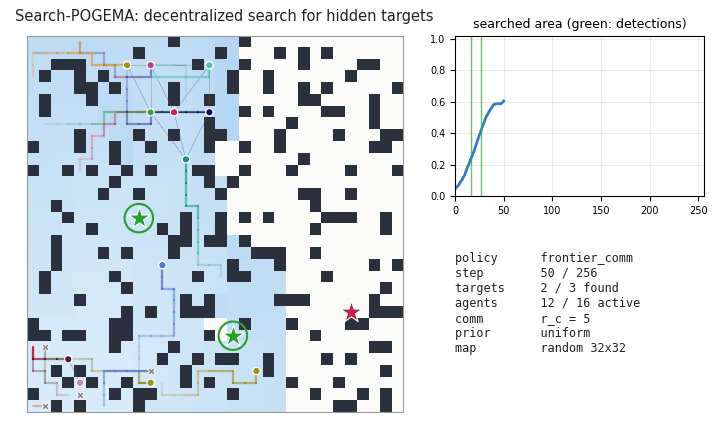
\includegraphics[width=0.72\linewidth]{../figures/task_frame.png}
\caption{Search-POGEMA episode (frontier exploration with map exchange, $r_c=5$): $32\times32$ map, 16 agents
deployed from one base, 3 hidden targets (red: hidden, green: detected), 25\% of agents failed (grey $\times$).
Blue: searched area, darker = later. Right: searched fraction over time with detection events.}
\label{fig:task}
\end{figure}
\textbf{Map and motion} come from POGEMA 1.3.1: random maps with obstacle density $\rho$ (POGEMA's generator), mazes
and warehouses (pogema-toolbox generators), five actions (stay/4 moves) and the \texttt{priority} collision system.
We use \texttt{on\_target='nothing'} because the default mode removes an agent when it reaches its POGEMA goal.
\textbf{Agents} start clustered around a random base (deployment from one point) inside the largest free component.
\textbf{Targets}: $K\in\{1,3\}$ cells of the same component that are not detectable at $t=0$, sampled uniformly or from
a Gaussian prior whose centre and width are known to the agents. \textbf{Sensing}: POGEMA's egocentric window
($r_o=3$, no line of sight); a target is detected when an active agent is within Chebyshev distance $r_d=2$.
\textbf{Memory}: each agent stores seen cells, known obstacles, searched cells (union of its detection footprints)
and visit counts; agents know their global position. \textbf{Communication}: agents within Euclidean distance $r_c$
merge their memories (OR / max), one hop per step; $r_c=0$ is no communication, $r_c=\infty$ global.
\textbf{Failures}: $\lfloor pN\rceil$ agents stop moving, sensing and communicating at a random step
$\sim\mathcal U[1,\,0.5\cdot\text{size}]$ and keep blocking their cell. The failure time is tied to the map size and not
to the episode limit, so failures hit every method \emph{during} the search (tying it to the time limit let fast
methods finish before most failures happened, which biased robustness estimates; we found and fixed this).
\textbf{Termination}: all targets detected or $T=8\cdot\text{size}$ steps.

\textbf{Metrics.} Success (all targets found); time to first / last detection, censored at $T$ and reported as a fraction
of $T$; coverage (searched fraction of the reachable area) and its AUC; team revisit ratio
$1-\#\text{distinct cells}/\#\text{agent-steps}$; messages and transmitted cells; robustness
$=\text{metric}(p)/\text{metric}(0)$. All aggregates are means with 95\% percentile-bootstrap CIs; every method sees
the same maps, starts, targets and failure schedules (paired design).

\section{Methods}
\textbf{Random walk}: uniform move among free neighbours. \textbf{L\'evy walk} \cite{viswanathan1999optimizing}: straight
flights of length $P(L)\propto L^{-\mu}$; $\mu=2$ was best on tuning seeds, matching theory.
\textbf{Frontier} \cite{yamauchi1997frontier,yamauchi1998multi}: each agent goes (BFS on its own known free cells) to the
nearest known free cell that is unsearched or borders unknown space, replanning on events (goal searched, new
obstacle, blocked by agents). \textbf{Frontier + maps}: same planner with memories merged within $r_c$.
\textbf{Frontier + allocation} (after \cite{burgard2005coordinated}): agents additionally broadcast their goal cell
to neighbours within $r_c$; agent $i$ minimises $d(c)+\lambda\sum_{g\in G_{<i}}\max(0,1-\|c-g\|_\infty/R)$ over
frontier cells, where $G_{<i}$ are goals announced by neighbours with a smaller id (decentralized analogue of the
sequential greedy assignment), with an exact best-first scan; $\lambda=0.1\cdot$size, $R=9$ selected on tuning seeds. \textbf{Swarm rule} (no communication): every step the agent takes
$\arg\max$ over free moves of
$w_g\,\text{gain}(c) - w_v\,\tfrac{v(c)}{1+v(c)} - w_r\sum_j\max(0,1-d(c,j)/R) + w_p'\cos(a,g) + w_m[a=a_{t-1}] + \epsilon$,
where gain is the share of new cells in the detection footprint, $v$ the agent's own visit count, $j$ the agents visible
in the POGEMA window (dispersion), $g$ the direction of the distance-weighted ``gravity''
$\sum_c p(c)e^{-d/\lambda}(c-x)/d^2$ of the unsearched prior mass, and $w_p'$ is boosted when no move has gain.
A plain centroid attraction failed (the centroid of the unsearched region falls into searched holes; single-agent
coverage 0.16 vs 0.74). Weights were selected on tuning seeds disjoint from evaluation seeds.
\textbf{IPPO} \cite{schulman2017ppo,dewitt2020independent}: one shared actor-critic (critic on the same local input). Input:
a $15\times15$ egocentric crop of the agent's own memory (7 channels), the whole map pooled to $8\times8$ (unsearched,
prior, obstacles, self; size-independent) and $t/T$; invalid moves are masked. Reward: $+1$ per own detection and
$0.02$ per prior-weighted reachable cell searched first in the team (ground truth used only for the training signal).
Time-limit ends are treated as terminal with $t/T$ in the input \cite{pardo2018time}. Curriculum $16\to32$ over random
densities, target counts, priors, failures and $r_c\in\{0,5\}$; 2.47M agent-steps ($\approx$45 min on 2 CPUs).
Checkpoint and stochastic action selection were chosen on tuning seeds (greedy $\arg\max$ loops; success 0.79).

\section{Experimental setup}
Full factorial grid with uniform targets on random maps: size $\{16,32,64\}$ $\times$ $\rho\{0,.1,.2,.3\}$ $\times$
$N\{4,8,16,32,64\}$ $\times$ $K\{1,3\}$ $\times$ $p\{0,.25,.5\}$; $r_c\in\{2,5,\infty\}$ for frontier+maps and
$\{0,\infty\}$ for IPPO; 10 evaluation seeds per cell (32\,400 episodes). Slices (10 seeds): Gaussian prior
(size 32/64, $\rho\in\{.1,.2\}$, $N\in\{8,16,32\}$, $p\in\{0,.5\}$) and maze / warehouse maps (same $N,p$).
Seeds: evaluation $0..19$, tuning $10^4+$, training $10^6+$. Code, configs, raw CSVs and figures are in the repository;
every number below is computed from those CSVs.

\section{Results}
\begin{table}[t]
\centering\small
\caption{Full grid, pooled over all 360 configurations (3\,600 episodes per method). Mean [95\% CI].}
\label{tab:leader}
\begin{tabular}{lcccccr}
\toprule
method & success & $t_{\text{last}}/T$ & $t_{\text{first}}/T$ & revisit & msgs/episode \\
\midrule
random walk & 0.461 [.444,.477] & 0.716 [.704,.727] & 0.477 & 0.825 & 0 \\
L\'evy walk & 0.740 [.725,.754] & 0.501 [.489,.514] & 0.294 & 0.692 & 0 \\
frontier & 0.868 [.857,.878] & 0.409 [.399,.420] & 0.229 & 0.675 & 0 \\
\textbf{swarm rule} & 0.900 [.890,.909] & \textbf{0.259} [.249,.269] & 0.142 & 0.463 & 0 \\
\textbf{IPPO} & 0.914 [.905,.922] & \textbf{0.259} [.250,.269] & 0.136 & 0.470 & 0 \\
\midrule
frontier + maps, $r_c=2$ & 0.951 [.944,.958] & 0.242 [.234,.250] & 0.134 & 0.481 & 1\,619 \\
frontier + maps, $r_c=5$ & 0.975 [.969,.980] & 0.194 [.187,.201] & 0.111 & 0.430 & 6\,026 \\
frontier + maps, global & 0.985 [.981,.989] & 0.178 [.172,.184] & 0.104 & 0.412 & 25\,483 \\
frontier + allocation, $r_c=5$ & 0.976 [.972,.981] & 0.200 [.194,.207] & 0.117 & 0.456 & 7\,459 \\
frontier + allocation, global & 0.989 [.986,.992] & \textbf{0.173} [.168,.178] & 0.104 & 0.424 & 28\,753 \\
IPPO, global (zero-shot) & 0.934 [.925,.942] & 0.223 [.214,.232] & 0.119 & 0.428 & 29\,011 \\
\bottomrule
\end{tabular}
\end{table}

\textbf{Without communication, swarm and IPPO tie and beat frontier.} Pooled over the grid (Table~\ref{tab:leader})
the swarm rule and IPPO have the same mean $t_{\text{last}}/T=0.259$ and are 1.6$\times$ faster than frontier without
communication, which sends agents to the same nearest frontiers: its revisit ratio is 0.68 vs 0.46--0.47. The
difference to frontier is largest on open maps: at $64\times64$, $\rho=0$, frontier needs 0.68 of the time limit vs
0.25 (swarm) and 0.27 (IPPO).
Fig.~\ref{fig:win} compares the two winners cell by cell with a paired test: the swarm rule is significantly faster
on $16\times16$ with 4--16 agents (paired difference $-0.061$ [$-0.103$, $-0.024$] at $N=4$), IPPO only at
$64\times64$, $N=8$ ($+0.080$ [$+0.013$, $+0.151$] in favour of IPPO), and all other cells are ties.
By map size, IPPO's advantage grows with the map ($t_{\text{last}}/T$ swarm vs IPPO: 0.083 vs 0.105 at 16,
0.195 vs 0.198 at 32, 0.359 vs 0.319 at 64), although 64$\times$64 was never seen in training.

\begin{figure}[t]
\centering
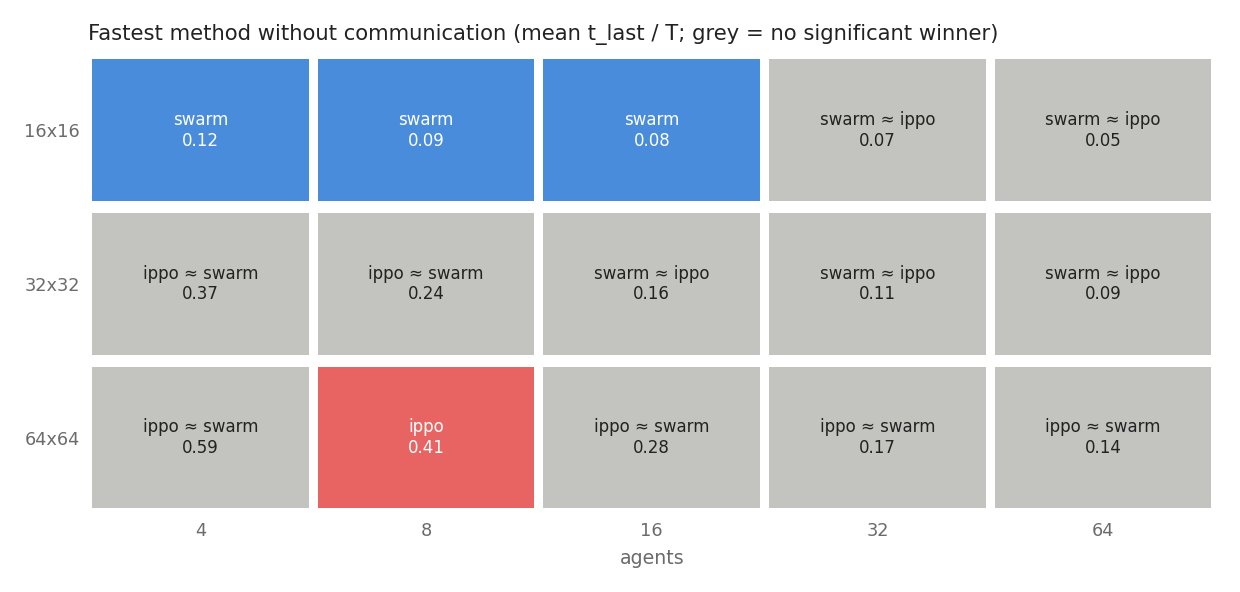
\includegraphics[width=0.62\linewidth]{../figures/full_winmap.png}
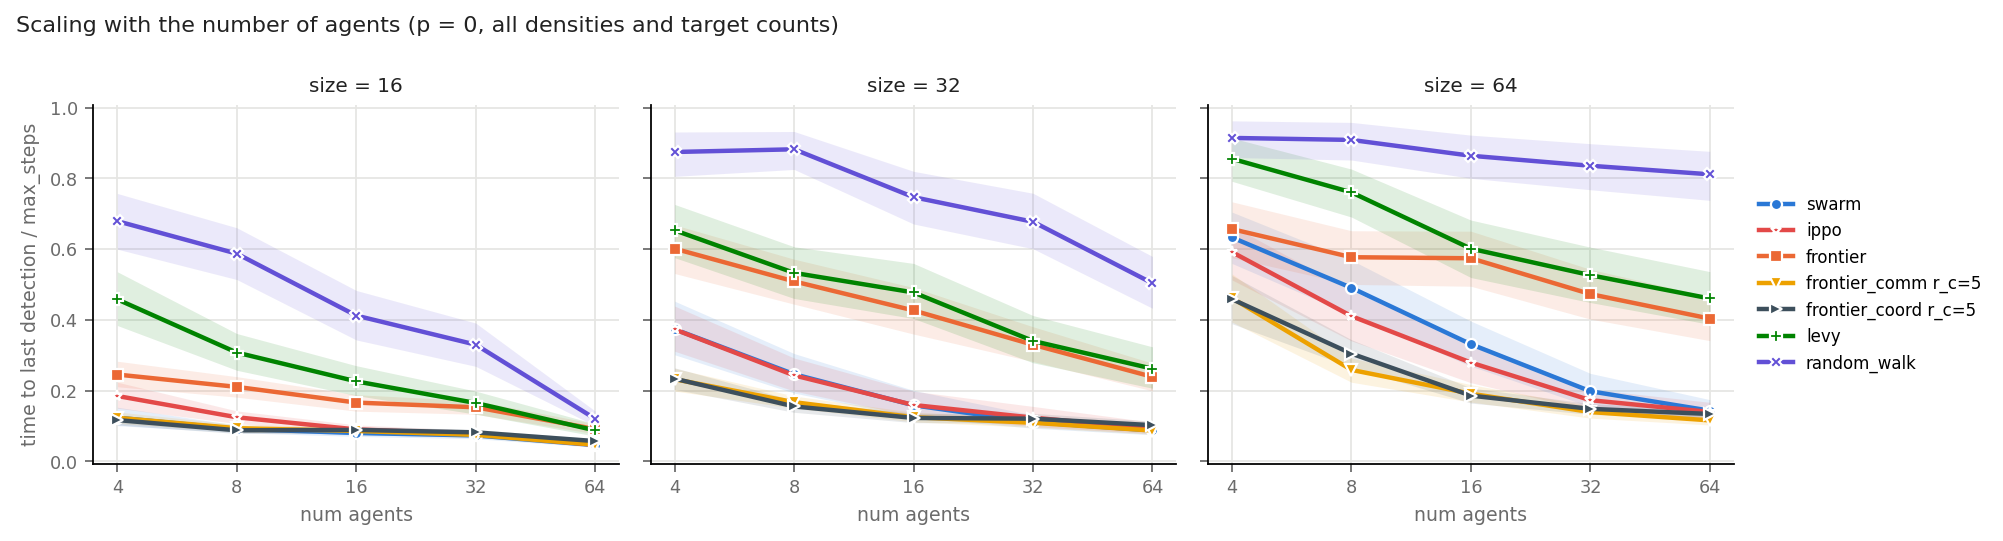
\includegraphics[width=0.98\linewidth]{../figures/full_scaling_agents.png}
\caption{Top: fastest communication-free method per (size, $N$), $p=0$; grey cells: the paired 95\% CI of the
difference to the runner-up contains 0. Bottom: $t_{\text{last}}/T$ vs number of agents (95\% CI bands).}
\label{fig:win}
\end{figure}

\textbf{Communication.} Map sharing is the strongest single factor (Fig.~\ref{fig:comm}). For frontier exploration,
$r_c=5$ recovers most of the benefit of global communication (0.154 vs 0.144 at $p=0$) with $\approx$21\% of its
messages; $r_c=2$ (0.195) is only slightly better than the communication-free swarm rule (0.213) while sending
$\approx$1\,900 messages per episode. IPPO, whose input is its own memory, profits from merged maps without
retraining (0.207 $\to$ 0.178) but less than frontier, whose planner exploits the shared map explicitly.
\textbf{Goal allocation} on top of map sharing is not a free win. With global communication it is the fastest method
overall (0.173 vs 0.178; paired difference $-0.005$ [$-0.008$, $-0.001$]), driven by $64\times64$ maps
($-0.016$ [$-0.024$, $-0.008$]) and slightly harmful on $16\times16$ ($+0.005$ [$+0.001$, $+0.008$]). With local
communication it is slightly worse ($r_c=5$: $+0.006$ [$+0.003$, $+0.010$]): an agent only sees the claims of its
nearest neighbours, and the penalty pushes it towards farther frontiers without a global picture. Its tuning on
4 seeds per setting suggested a large gain at $64\times64$, $N=8$ (0.46 vs 0.65) that did not replicate on the
evaluation seeds (0.305 vs 0.259) --- a reminder that small tuning sets overfit.

\begin{figure}[t]
\centering
\begin{subfigure}{0.49\linewidth}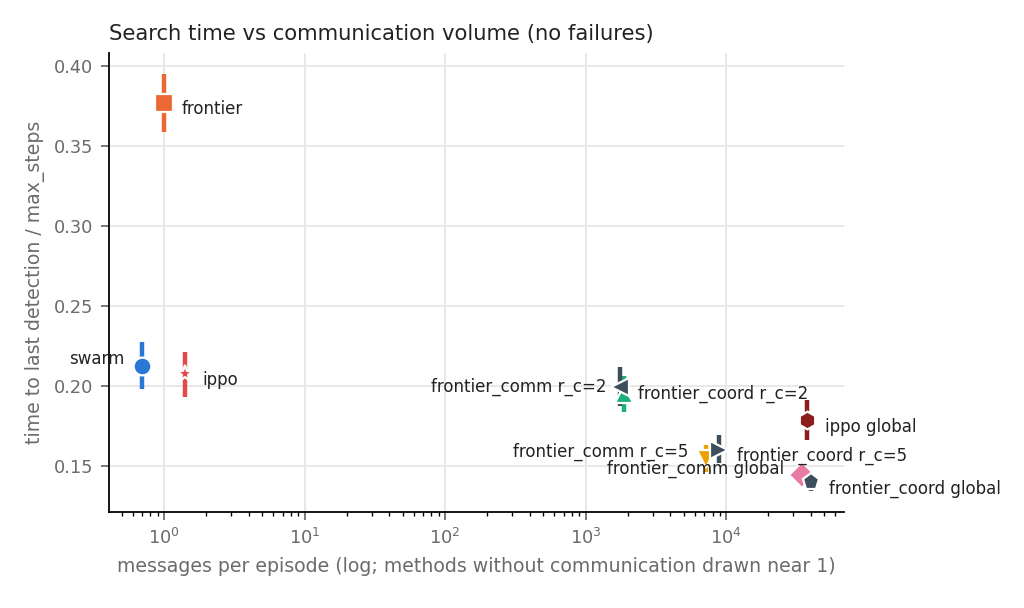
\includegraphics[width=\linewidth]{../figures/full_comm_tradeoff.png}\end{subfigure}
\begin{subfigure}{0.49\linewidth}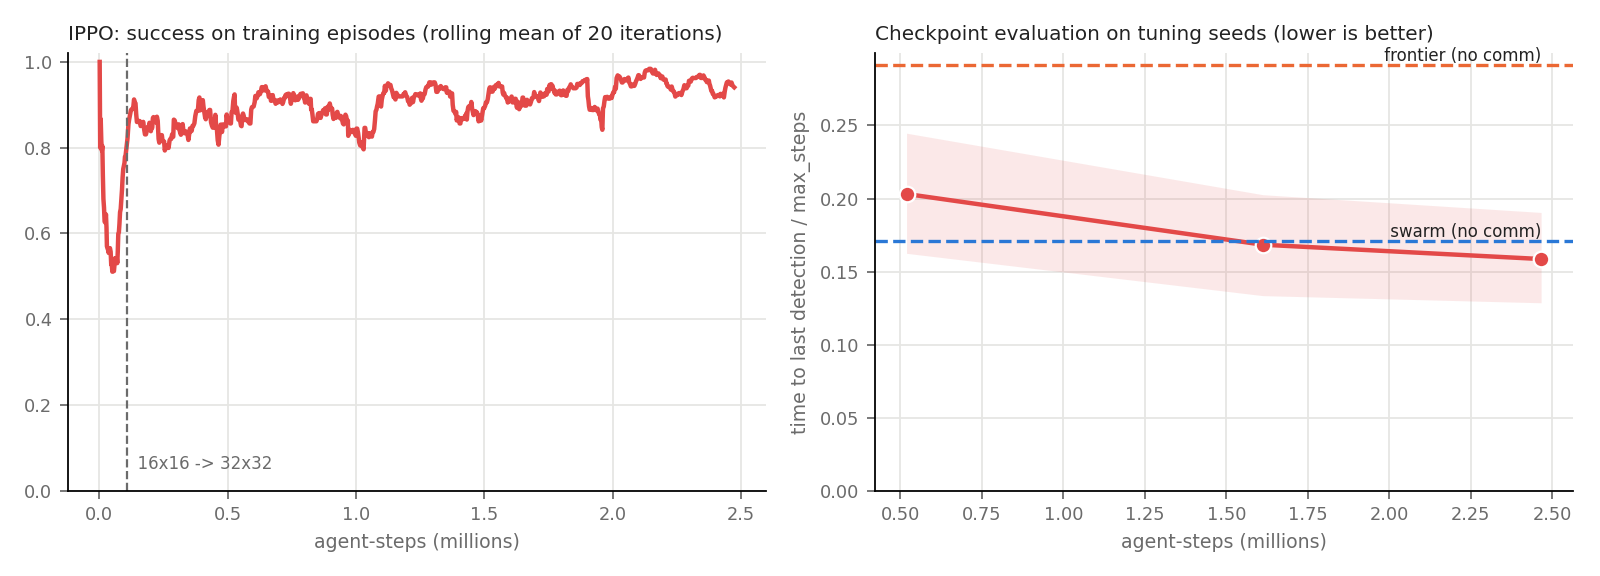
\includegraphics[width=\linewidth]{../figures/stage3_learning_curve.png}\end{subfigure}
\caption{Left: search time vs messages per episode ($p=0$, pooled). Right: IPPO training (success on training
episodes; checkpoint evaluation on tuning seeds vs the swarm rule and frontier).}
\label{fig:comm}
\end{figure}

\textbf{Robustness.} Losing 50\% of the agents increases $t_{\text{last}}$ by $\times$1.44 [1.31, 1.58] for the swarm
rule, $\times$1.54 [1.41, 1.69] for IPPO and $\times$1.60 [1.47, 1.73] for frontier + maps ($r_c=5$); success drops to
0.87, 0.86 and 0.95. Relative ratios favour slow methods (random walk $\times$1.12) because their baseline is already
near the limit, so we read robustness together with absolute success: at $64\times64$, $p=0.5$, success is 0.74
(swarm), 0.76 (IPPO) and 0.89 (frontier, $r_c=5$) --- with failures, redundancy through map sharing matters most on large maps.

\begin{table}[t]
\centering\small
\caption{Slices: $t_{\text{last}}/T$, mean [95\% CI], pooled over the slice (episodes per method: 240 prior, 120 maze, 120 warehouse).}
\label{tab:slices}
\begin{tabular}{lccc}
\toprule
method & Gaussian prior & maze & warehouse \\
\midrule
frontier & 0.507 [.467,.548] & 0.635 [.581,.687] & 0.625 [.566,.681] \\
swarm rule & \textbf{0.164} [.148,.181] & 0.470 [.406,.532] & 0.275 [.241,.313] \\
IPPO & 0.174 [.158,.191] & 0.421 [.367,.477] & 0.302 [.265,.342] \\
frontier + maps, $r_c=5$ & 0.227 [.202,.253] & 0.247 [.219,.278] & 0.223 [.197,.252] \\
frontier + maps, global & 0.178 [.162,.195] & 0.218 [.197,.242] & 0.187 [.169,.205] \\
frontier + allocation, global & 0.168 [.154,.183] & \textbf{0.216} [.198,.237] & \textbf{0.183} [.168,.198] \\
IPPO, global & \textbf{0.143} [.128,.159] & 0.390 [.337,.447] & 0.220 [.190,.252] \\
\bottomrule
\end{tabular}
\end{table}

\textbf{Priors and structured maps} (Table~\ref{tab:slices}). With a known target prior the communication-free swarm
rule (0.164) is as fast as frontier with global map sharing (0.178), because frontier ignores the prior while the swarm
rule's weak attraction concentrates agents where targets are likely; IPPO with global maps is the fastest (0.143).
In mazes the picture flips: without a shared map, agents repeatedly enter the same dead ends, and frontier + maps
($r_c\ge5$) is 1.7--1.9$\times$ faster than the communication-free methods. Warehouses are in between.

\textbf{How far from optimal?} For the $64\times64$ episodes ($p=0$) we compute a per-episode lower bound on
$t_{\text{last}}$: the larger of the travel bound (the last target must be reached from the base,
$\max_k\min_i$ BFS distance to its detection zone) and an area bound (at most $2r_d+1$ new cells per agent and
step). In successful episodes the median ratio $t_{\text{last}}/\text{LB}$ is 1.51 for frontier + maps ($r_c=5$),
1.54 for frontier + allocation (global), 1.65 for the swarm rule, 1.67 for IPPO, 3.43 for frontier, 4.02 for
L\'evy and 6.60 for the random walk (medians over successful episodes favour methods that fail on hard episodes).
The large mean $t_{\text{last}}/T$ of the swarm rule at $64\times64$ (0.36) is mostly due to failures: 40\% of it comes
from the 14.5\% unsolved episodes, concentrated at density 0.3 (success 0.57) and few agents, where a purely
local rule cannot leave dead-end pockets.

\section{Discussion and limitations}
A tuned local rule with three ingredients --- dispersion, own-memory novelty and a weak prior pull --- matches a learned
IPPO policy and beats uncoordinated frontier exploration when there is no communication; learning pays off on larger
maps and transfers zero-shot to bigger maps and to shared memories. Limitations: (1) IPPO was trained for only 2.5M
agent-steps and only up to $32\times32$; longer training, a $64\times64$ phase or MAPPO / a recurrent policy may change
the ranking. (2) The swarm weights were tuned on 32 episodes per setting, and the allocation parameters on 4 seeds per setting
(which overfit, see above); a centralized or auction-based allocation could still be stronger than our
decentralized priority scheme.
(3) Sensing has no line of sight and agents know their global position; agents cannot tell failed robots from active
ones. (4) 10 seeds per cell; CIs are per cell and pooled, without multiple-comparison correction.
Next steps: a hybrid in which a high-level swarm/frontier rule chooses subgoals and a pretrained POGEMA policy
(Follower \cite{skrynnik2024follower} or MAPF-GPT \cite{andreychuk2025mapfgpt}) moves the agents; and IPPO with
learned message passing under a communication budget.

\small
\begin{thebibliography}{10}
\bibitem{skrynnik2025pogema} A.~Skrynnik, A.~Andreychuk, A.~Borzilov, A.~Chernyavskiy, K.~Yakovlev, A.~Panov.
POGEMA: A Benchmark Platform for Cooperative Multi-Agent Pathfinding. \emph{ICLR}, 2025.
\bibitem{skrynnik2024follower} A.~Skrynnik, A.~Andreychuk, M.~Nesterova, K.~Yakovlev, A.~Panov. Learn to Follow:
Decentralized Lifelong Multi-Agent Pathfinding via Planning and Learning. \emph{AAAI}, 2024.
\bibitem{andreychuk2025mapfgpt} A.~Andreychuk, K.~Yakovlev, A.~Panov, A.~Skrynnik. MAPF-GPT: Imitation Learning for
Multi-Agent Pathfinding at Scale. \emph{AAAI}, 2025.
\bibitem{yamauchi1997frontier} B.~Yamauchi. A frontier-based approach for autonomous exploration. \emph{IEEE CIRA}, 1997.
\bibitem{yamauchi1998multi} B.~Yamauchi. Frontier-based exploration using multiple robots. \emph{Agents}, 1998.
\bibitem{burgard2005coordinated} W.~Burgard, M.~Moors, C.~Stachniss, F.~Schneider. Coordinated multi-robot exploration.
\emph{IEEE Trans. Robotics}, 21(3), 2005.
\bibitem{viswanathan1999optimizing} G.~M.~Viswanathan et al. Optimizing the success of random searches. \emph{Nature}, 401, 1999.
\bibitem{schulman2017ppo} J.~Schulman et al. Proximal policy optimization algorithms. arXiv:1707.06347, 2017.
\bibitem{dewitt2020independent} C.~Schroeder de Witt et al. Is independent learning all you need in the StarCraft
multi-agent challenge? arXiv:2011.09533, 2020.
\bibitem{pardo2018time} F.~Pardo, A.~Tavakoli, V.~Levdik, P.~Kormushev. Time limits in reinforcement learning. \emph{ICML}, 2018.
\end{thebibliography}
\end{document}
